%設定頁面
\documentclass[12pt,a4paper]{article}
\usepackage[margin=1in,a4paper]{geometry}

%設定中文
\usepackage{xeCJK} 
\setCJKmainfont{標楷體} 
\XeTeXlinebreaklocale "zh"   
\XeTeXlinebreakskip = 0pt plus 1pt 

%浮水印
%\usepackage{draftwatermark}
%\SetWatermarkText{\bf NTNU MATH}
%\SetWatermarkScale{0.7}

%圖片
\usepackage{graphicx}
\usepackage{subfigure}

%頁首頁尾
\makeatother
\usepackage{fancyhdr}

%顏色
\usepackage{xcolor}

%表格顏色
\usepackage{colortbl}

%設定數學
\usepackage{amsmath, amsthm, amssymb}
\makeatletter

%自定圈圈標號
\usepackage{pstricks,pstricks-add}
\newcommand\textc[1]{{\begin{pspicture*}
(-0.25,-0.2)(0.25,0.3)\rput[c](0,0)
{\large \textcircled{\footnotesize #1}}
\end{pspicture*} }}

%自訂向量符號
\def\leftharpoonfill@{\arrowfill@\leftharpoonup\relbar\relbar}
\def\rightharpoonfill@{\arrowfill@\relbar\relbar\rightharpoonup}
\newcommand\rbjt{\mathpalette{\overarrow@\rightharpoonfill@}}
\newcommand\lbjt{\mathpalette{\overarrow@\leftharpoonfill@}}

%自訂定理
\newtheorem*{thm}{Theorem}
\newtheorem*{lem}{Lemma}
\newtheorem*{de}{Definition}
\newtheorem*{rmk}{Remark}
\newtheorem*{ex}{Example}
\newtheorem*{pf}{Proof}
\newtheorem*{sol}{Solution}

%程式碼
\usepackage{listings}
\usepackage{color}

\definecolor{dkgreen}{rgb}{0,0.6,0}
\definecolor{gray}{rgb}{0.5,0.5,0.5}
\definecolor{mauve}{rgb}{0.58,0,0.82}

\lstset{
  basicstyle={\small \ttfamily},
  frame=tb,
  language=Python,
  aboveskip=3mm,
  belowskip=3mm,
  showstringspaces=false,
  columns=flexible,
  basicstyle={\small\ttfamily},
  numbers=left,
  numbersep = 14pt,
  numberstyle=\tiny\color{gray},
  keywordstyle=\color{blue},
  commentstyle=\color{dkgreen},
  stringstyle=\color{mauve},
  breaklines=true,
  breakatwhitespace=true,
  tabsize=3,
  backgroundcolor=\color{gray!10}
}




%作者
\title{NTNU影像處理HW5}
\author{廖家緯}
\date{2020.4.15}

\begin{document}
\maketitle
%標題、作者、日期
\fontsize{12pt}{20pt}\selectfont
%設定字體大小、間距
\setlength{\baselineskip}{20pt}
%設定行距

\pagestyle{fancy}
\lhead{}
\chead{}
\rhead{}
\lfoot{}
\cfoot{\thepage}
\rfoot{}
\renewcommand{\headrulewidth}{0pt} %上線寬
\renewcommand{\footrulewidth}{0pt} %下線寬
%\renewcommand{\abstractname}{Executive Summary}




%正文開始
\begin{enumerate}
\item[•]{\bf Outline}:
\begin{enumerate}
\item[1.]CalSelect an experimental image
\item[2.]
Apply a 3 by 3 (a) average filter and
(b) median filter to the image
\item[3.]
Unsharp masking\\
\begin{figure}[h]
\hspace*{5em}
\begin{tabular}{c}
\includegraphics[height=1.2in]{img1.jpg}
\end{tabular}
\end{figure}\\
\end{enumerate}

\item[•]
{\bf Code(Python):}
\begin{lstlisting}
import numpy as np
import cv2

# 讀取灰階影像
I = cv2.imread('image.jpg', cv2.IMREAD_GRAYSCALE)

# 周圍補0
I1 = np.pad(I,((1,1),(1,1)),'constant',constant_values = (0,0))
N = np.shape(I1)[0]
M = np.shape(I1)[1]

# Average filter 和 Median filter
I2 = np.zeros((N, M), int).astype('double')
I3 = np.zeros((N, M), int).astype('uint8')

for i in range(1, N-1):
    for j in range(1 ,M-1):
        I2[i,j] =  I1[i-1:i+2, j-1:j+2].mean()
        I3[i,j] =  sorted(I1[i-1:i+2, j-1:j+2].reshape(9))[4]

I2 = I2.astype('uint8')  # 經過 Average filter 掃過的影像
I3 = I3.astype('uint8')  # 經過 Median filter 掃過的影像

# Unsharp masking
k = 0.4
s = 1/(1-k)
I4 = ((I1 - k*I2)*s).astype('uint8')
I5 = ((I1 - k*I3)*s).astype('uint8')

\end{lstlisting}

\item[•]
{\bf Input image:}\\
\begin{figure}[h]
\hspace*{11em}
\begin{tabular}{c}
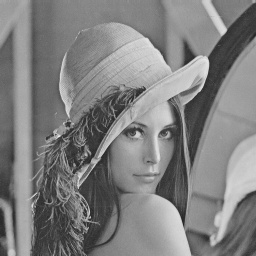
\includegraphics[height=2.4in]{Gray.jpg}\\
Original
\end{tabular}
\end{figure}

\item[•]
{\bf Result:}
\begin{figure}[h]
\hspace*{3em}
\begin{tabular}{cc}
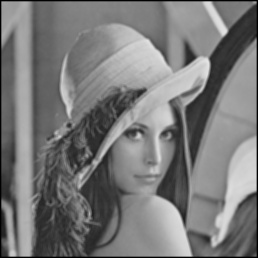
\includegraphics[height=2.4in]{average_filter.jpg}&
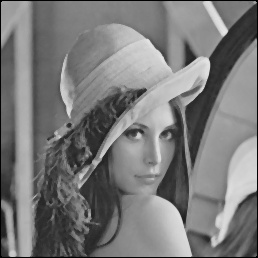
\includegraphics[height=2.4in]{median_filter.jpg}\\
Average filter  & Median filter \vspace*{2em}\\
\end{tabular}
\end{figure} 

\newpage
\begin{figure}[h]
\hspace*{3em}
\begin{tabular}{cc}
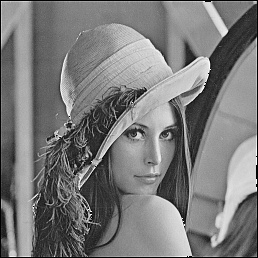
\includegraphics[height=2.4in]{average_filter_us.jpg}&
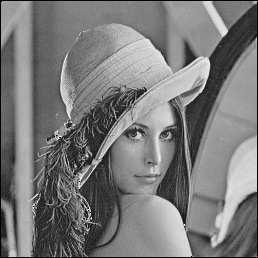
\includegraphics[height=2.4in]{median_filter_us.jpg}\\
Unsharp Masking by average filter &
Unsharp Masking by median filter \\
\end{tabular}
\end{figure} 

\item[•]
{\bf Experience:}\\
在這次作業中,average filter 和 median filter 的製作原本可能需要4層迴圈,我使用numpy直接對矩陣逐項計算,因此減少到只需2層迴圈,大幅降低了時間複雜度。而處理 Unsharp masking,我嘗試了不同的$k$,最後選用看起來比較完美的$0.4$,我們可以發現,經過 Unsharp masking 後,頭髮與眼睛的輪廓變得比較明顯。另外,為了擔心 Unsharp masking 後的影像會變得太暗,我根據課本提供的方法,乘上$s$值來調整明暗程度(課本$k$剛好與我的成倒數,因此我將公式重新調整過)。
\end{enumerate}










\end{document}